\chapter{LED ĐƠN}
\label{Les:1}
\section{Giới thiệu chung}
\subsection{Yêu cầu}
Điều khiển các chân \verb|I/O| của PIC 16F887 với chức năng \verb|OUTPUT| thông qua chóp tắt các LED được nối với PORT E của vi điều khiển.
\subsection{LED}
LED là diode có khả năng phát ra ánh sáng hay tia hồng ngoại, tia tử ngoại. Có điện thế phân cực thuận từ $1.5 \div 3V$, điện thế phân cực ngược thấp.

Điện thế phân cực thuận của một số loại LED:
\begin{table}[!h]
\begin{center}
\begin{tabular}{|p{2.3cm}|c|}\hline
\centering{\textbf{Loại LED}} & \textbf{Điện thế phân cực thuận} \\ \hline
Đỏ & $1.4 \div 1.8V$\\ \hline
Vàng & $2.0 \div 2.5V$\\ \hline
Xanh lá cây & $2 \div 2.8V$\\ \hline
\end{tabular}
\end{center}
\caption{Điện thế phân cực thuận của một số LED}
\end{table}

Với các loại LED thường thì: $I_{max} = 30mA$. Còn LED loại siêu sáng thì điện áp phân cực thuận cao hơn LED thường (có loại lên đến $5V$), dòng $I_{max} = 30mA$.\\

Cách mắc điện trở hạn dòng cho LED:
\begin{list}{--}{}
\item Có $n$ LED mắc nối tiếp nhau:
\begin{align*}
R_{nt} = \frac{U_{\text{\textit{nguồn}}} - n \times U_{LED}}{I_{max}}
\end{align*}
\item Có $m$ nhánh đấu mắc song song (mỗi nhánh gồm $n$ LED nối tiếp):
\begin{align*}
R_{ss} = \frac{R_{nt}}{m}
\end{align*}
\item[$\ast$] Tùy theo yêu cầu về độ sáng của LED mà ta chọn giá trị của điện trở cho phù hợp.
\end{list}
\subsection{Sơ đồ mạch}
\begin{figure}[!h]
\begin{center}
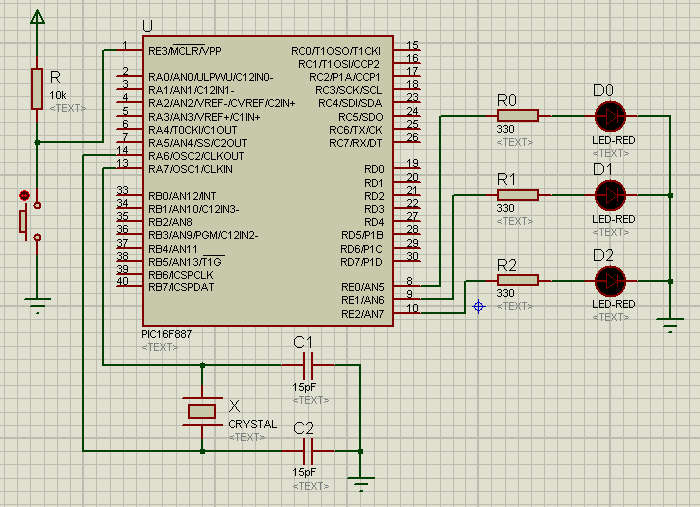
\includegraphics[scale=0.7]{bai-1/image/BAI-1}
\end{center}
\caption{Mạch điều kiển LED nối với PORT E}
\end{figure}
\section{Cách điều khiển các chân xuất nhập số}
PORT E có chức năng xuất nhập số \verb|I/O| và chức năng chuyển đổi \verb|ADC|. Ở đây chúng ta quan tâm đến chức năng xuất nhập số.
\paragraph{Cách điều khiển:}
\begin{itemize}
\item Xác định các chân của PORT E là chân \verb|OUTPUT| hay là \verb|INPUT|, dùng lệnh: \verb|TRISA| hoặc \verb|TRISB| hoặc \verb|TRISC| hoặc \verb|TRISD| hoặc \verb|TRISE|, ở đây mình điều khiển PORT E nên dùng \verb|TRISE|.
\begin{itemize}
\item Mỗi chân sẽ có một trạng thái là \verb|0| (chân \verb|OUTPUT|) hoặc \verb|1| (chân \verb|INPUT|).
\item Cả ba chân \verb|RE2, RE1, RE0| là chân \verb|OUTPUT| thì: \verb|TRISE = 0b000 = 0x00|, thứ tự bit là \verb|RE2-RE1-RE0| (tương tự như các PORT khác, theo thứ tự là chân có chỉ số cao đến chân có chỉ số thấp).

Ví dụ: \verb|RE2 - INPUT|, \verb|RE1,RE0 - OUTPUT| thì: \verb|TRISE = 0b100 = 0x04|, tương tự như các trường hợp khác của các PORT còn lại.
\item Để đơn giản cho việc lập trình, chúng ta có thể khai báo mã ở dạng nhị phân \verb|0b...| hoặc khai báo mã dạng thập lục phân \verb|0x...| (mã hex).
\end{itemize}
\item Nếu là chân \verb|OUTPUT| thì dùng \verb|0| (mức thấp) hoặc \verb|1| (mức cao) để thể hiện trạng thái của một chân.

Ví dụ: \verb|RE2,RE1,RE0| -- chân \verb|OUTPUT| ở mức cao thì: \verb|PORTE = 0b111 = 0x07|; \verb|RE2| -- chân \verb|OUTPUT| ở mức cao, \verb|RE1,RE0| -- chân \verb|OUTPUT| ở mức thấp thì: \verb|PORTE = 0b100| \verb|= 0x04| 
\item Nếu là chân \verb|INPUT|, thì phải đọc tín hiệu của chân đó (được xét ở bài sau).
\item Một số hàm hổ trợ: \verb|delay_ms(số mili giây)| hoặc \verb|delay_us(số micro giây)|, các cấu trúc lập trình \verb|for, while, if, if ... else,|\ldots
\end{itemize}
\section{Bài tập}
Trong chương trình có sử dụng thư viện \verb|DEF_887.H| (trong \emph{phụ lục \ref{def:887} trang \pageref{def:887}}).
\subsection{Bài tập 1.1}
\paragraph{Yêu cầu}Viết chương trình chóp tắt LED ở PORT E với thời gian delay $250ms$.
\paragraph{Hướng giải quyết} 
\begin{itemize}
\item Khai báo các chân ở PORT E là chân \verb|OUTPUT|: \verb|TRISE = 0x00|.
\item Lặp lại quá trình sau (dùng cấu trúc \verb|while|): LED tắt (\verb|PORTE = 0x00|); giữ trạng thái cũ $250ms$ (\verb|delay_ms(250)|); LED sáng (\verb|PORTE = 0b111 = 0x07|); giữ trạng thái cũ $250ms$ (\verb|delay_ms(250)|). Theo cách lập trình này ta có \textit{Chương trình 1}.
\item[$\ast$] \textit{Cách khác}: đầu tiên cho LED tắt (\verb|PORTE = 0x00|). Lặp lại quá trình: đảo trạng thái của LED (\verb|PORTE = | $\sim$\verb|PORTE|); giữ trạng thái cũ $250ms$ (\verb|delay_ms(250)|). Theo cách lập trình này ta có \textit{Chương trình 2}.
\end{itemize}
\newpage
\subsection*{Chương trình 1}
\lstinputlisting[language=C]{BAI-1-1.C}
\subsection*{Chương trình 2}
\lstinputlisting[language=C]{BAI-1-1v2.C}
\newpage
\subsection{Bài tập 1.2}
\paragraph{Yêu cầu}Viết chương trình chóp tắt LED ở PORT E với thời gian delay $1s$.
\paragraph{Hướng giải quyết} Ta sử dụng hàm \verb|delay_ms(số mili giây)| với tham số truyền vào là $1000$. Hàm \verb|delay_ms(số mili giây)| có tham số \verb|'số mili giây'| có giá trị $0 - 65535$ (\verb|int16|).
\paragraph{Chương trình}Sử dụng lại \textit{Chương trình 1} hoặc \textit{Chương trình 2}, thay đổi \verb|delay_ms(250)| thành \verb|delay_ms(1000)|.
\subsection{Bài tập 1.3}\label{Exe:1-3}
\paragraph{Yêu cầu}Viết chương trình chóp tắt LED ở chân \verb|RE1| với thời gian delay $1s$ và LED ở chân \verb|RE2| với thời gian delay là $0.5s$.
\paragraph{Hướng giải quyết}
\begin{itemize}
\item Với yêu cầu thì 2 LED thực hiện chóp hoặc tắt cùng một lúc khi mới vào chu kỳ đầu, nhưng phải đảm bảo đúng được chu kỳ của mỗi LED, với thời gian delay khác nhau, nên chia ra các trường hợp sau (để đảm bảo đúng thời gian \verb|delay|):
\begin{center}
\begin{tabular}{|c|c|c|c|}\hline
Thời gian & LED ở \verb|RE2| & LED ở \verb|RE1| & \verb|PORTE| \\ \hline
$0ms$ & \verb|ON| & \verb|ON| & \verb|0b110 = 0x06|\\ \hline
$500ms$ & \verb|OFF| & \verb|ON| & \verb|0b010 = 0x02|\\ \hline
$1000ms$ & \verb|ON| & \verb|OFF| & \verb|0b100 = 0x04| \\ \hline
$1500ms$ & \verb|OFF| & \verb|OFF| & \verb|0b000 = 0x00| \\ \hline
$2000ms$ & \multicolumn{3}{c|}{Lặp lại trạng thái}\\ \hline
\end{tabular}
\end{center}
\item Dựa vào bảng trên, ta viết được \emph{chương trình 3} thỏa yêu cầu.
\end{itemize}
\newpage
\subsection*{Chương trình 3}
\lstinputlisting[language=C]{BAI-1-3.C}

